\cotefile{75}
\scanpage{2}
% margin note written sideways in the scan, parallel to the title
\margin{(24 p)}
$C_{4}$\qquad DEA

\unsure{Géométries|Géometries} Combinatoires
% archive sheet number: 1
\scanpage{3}
\uline{Rappels de théorie des groupes} \uline{et sur espaces homogènes}

Groupe (loi comp. assoc. unitaire avec inverses)

hom de groupes (on a néc $f(e)=e$, $f(x^{-1})=f(x)^{-1}$)

opération d'un groupe $G$ sur un ens (ens. à groupe d'opérateurs)

opération transitive ($\forall x\unsure{,|\mathord{.}}y\in E,\ \exists g\in G,\ y=gx$) -- espace homogène

On exige \inserted{de plus} que $E\ne\varnothing$)
\[
\bigl(\text{couples }(E,x),\ E\ \text{esp. hom.},\ x\in E\bigr)
\Longleftrightarrow
\begin{aligned}&\text{donnée d'un ss-grpe}\\&H\ \text{de }G\end{aligned}
\]

c'est en fait une ``équivalence de catégories''

% slanted
\margin{classes d'iso. d'esp. hom. ss $G$ $\unsure{\simeq|\sim}$ classes de conjugaison de ss-grpes}
{\small
\diagram{\begin{tikzcd}[ampersand replacement=\&,row sep=0.6em,column sep=0.8em]
(E,x) \arrow[dd,"f"] \& \& \& {}\\
{} \& (f(x)=x') \& \Longleftrightarrow \& H\subset H'\\
(E',x') \& {\begin{aligned}&\text{\uline{NB} }f\ \text{(\unsure{comm.|compat.} à }G\text{) connu,}\\&\text{quand on \unsure{connaît|connait}}\\& f(x),\ \text{\uline{si} }G\ \text{trans. sur }E\end{aligned}} \& \& {}
\end{tikzcd}}}
{\small
\[
\begin{aligned}
E\sim E' \quad &\text{sss}\quad H,H'\ \text{conjugués}\quad \big/\\[-2pt]
&\exists E\to E'\quad\text{sss}\quad H\ \text{conjugué à un ss-grpe de }H'
\end{aligned}
\]}

\uline{Torseur sous $G$} :
{\small
\diagram{\begin{tikzcd}[ampersand replacement=\&,row sep=1.25em,column sep=1.5em]
{\left\{\begin{aligned}&\forall x,y\in E,\quad\exists 1\ g\in G,\quad gx=y\\& E\ne\varnothing\end{aligned}\right\}}
\arrow[r,Leftrightarrow] \arrow[d,Leftrightarrow] \&
{\left\{\begin{aligned}&E\ \text{espace hom.,}\\&\text{stabilisateur}\\&\text{des pts réd.}\\&\text{à }\{e\}\end{aligned}\right\}}\\
{\left\{E\simeq G_{s}\right\}} \&
\end{tikzcd}}}

\deleted{\unsure{Les|Le}}

Les torseurs sous $G$ sont isomorphes (non canoniquement)

Les torseurs sous $G$ sont les ``plus gros'' espaces homogènes ss $G$.

\unsure{Le|le} groupe des autom. d'un torseur $P$ sous $G$ est $\sim G$ (non canonique) : le choix de $x\in P$ définit un iso. $G\overset{u_x}{\simeq}\operatorname{Aut}_{G}P$, si on remplace $x$ par \inserted{$y=$}$gx$, cet iso. est remplacé par
\[
\boxed{u_y=u_{\unsure{g|s}x}=\deleted{\unsure{\operatorname{int}(g)\circ|\operatorname{int}g\circ}}u_x\unsure{\circ\,?|\circ}\operatorname{int}(s^{-1})}
\]
{\small
\[
\begin{aligned}
\bigl[\,u_x(g).\,x=gx\qquad &u_y(g)y=gy=gsx\unsure{=|.}\\
&\quad\unsure{\Vert|\text{''}}\\[-3pt]
&u_y(g)sx=s\,u_y(g)x
\\
&\hspace{1em}\deleted{\unsure{\Leftarrow ?|\Leftrightarrow ?}} \qquad u_y(g).\,x=s^{-1}gs\,x\\
&\hspace{9.4em}=u_x(s^{-1}gs).\,x\\
&\deleted{\bigl(u_x\circ\operatorname{int}(s)\bigr)(g)y=u_x(sgs^{-1})(y)=}\\
&u_y(g)=u_x(s^{-1}gs)\hspace{3em}\bigr]
\end{aligned}
\]}
% archive sheet number: 2
\scanpage{4}
\deleted{\unsure{Rappel|Rapp.}}

\uline{Graphes}

\[
\begin{aligned}
\text{\uline{\unsure{Def|Déf}}}\\[-2pt]\text{\uline{Graphe}}
\end{aligned}
\quad
\left\{\begin{aligned}
&\text{Ens } S\ \text{de ``sommet''}\\
&\text{ens } A\ \text{``d'arêtes''}\\
&R\subset S\times A\qquad\text{relation d'incidence}
\end{aligned}\right\}
\ \text{Données}
\]

\uline{\unsure{Axiome|Axiomes}} \quad 1) $\forall a\in A,\ \unsure{\exists|\exists s}\ \operatorname{card}R\{a\}=2$ (tte arête a exactement 2 \unsure{sommet|sommets})

\noindent\begin{minipage}[t]{.32\linewidth}
\figure{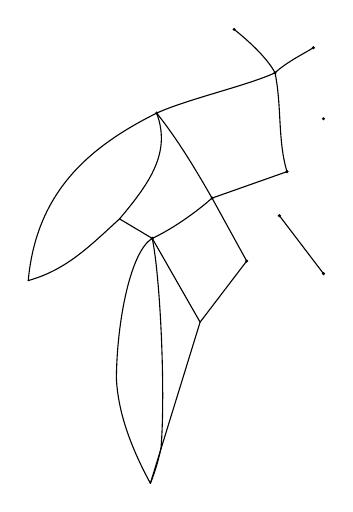
\begin{tikzpicture}[x=.008cm,y=-.008cm,line cap=round,line join=round]
\draw (492,496) .. controls (511,511) and (544,540) .. (557,565)
  .. controls (575,548) and (604,534) .. (618,525);
\draw (557,565) .. controls (514,585) and (417,607) .. (369,629)
  .. controls (263,682) and (178,753) .. (165,895);
\draw (165,895) .. controls (226,878) and (263,840) .. (310,797)
  .. controls (359,739) and (392,691) .. (369,629);
\draw (369,629) .. controls (404,673) and (431,719) .. (457,764)
  -- (576,722) .. controls (561,672) and (568,619) .. (557,565);
\draw (310,797) -- (362,828) .. controls (394,813) and (431,787) .. (457,764)
  -- (512,864) -- (438,961) -- (362,828);
\draw (362,828) .. controls (328,848) and (306,957) .. (305,1050)
  .. controls (308,1116) and (338,1178) .. (359,1217);
\draw (362,828) .. controls (375,891) and (383,1071) .. (376,1160)
  .. controls (371,1185) and (365,1202) .. (359,1217);
\draw (438,961) -- (359,1217);
\draw (564,792) -- (634,884);
\foreach \x/\y in {492/496,618/525,557/565,369/629,576/722,457/764,362/828,512/864,564/792,634/884,634/638}
  \fill (\x,\y) circle[radius=2.7];
\end{tikzpicture}}
\end{minipage}\hfill
\begin{minipage}[t]{.63\linewidth}
Un graphe est dit \deleted{\unsure{qqch|quelq.}} \uline{strict} si une arête est connue quand on connait ses sommets.

\deleted{\unsure{On|Un}} La donnée d'un \uline{graphe strict} équivaut donc \unsure{à la|à 2} donnée d'un ens. $S$, et d'une partie $A$ de $\unsure{\mathfrak{P}|\mathcal{P}}_{2}(S)$ (ens des parties de card. 2 de $S$).
\end{minipage}

\unsure{Arc|Arcs} d'un graphe (ou arête orientée) -- ens $\vec A$

\deleted{\uline{\unsure{Remarque}}} Réalisation topologique d'un graphe
\[
\deleted{X(S,A,R)=\bigl(S\amalg(\vec A\times I)\bigr)/\unsure{.}}
\]

a) Segment associé à un ens $a$ de card. 2
\[
\begin{aligned}
\bigl[\,\deleted{\unsure{\operatorname{réal}|\operatorname{rel}}}\inserted{\operatorname{seg}}(a)&\subset I^{a}\qquad (I=[0,1])\\
\operatorname{seg}(a)&=\bigl\{\{t_x\}_{x\in a}\mid\textstyle\sum t_x=1\bigr\}\ ;\ \text{on a }\ a\hookrightarrow\operatorname{seg}(a)
\end{aligned}
\]

b)
\[
\operatorname{réal}(S,A,R)=\left(S\amalg\coprod_{a\in A}\operatorname{seg} R\{a\}\right)\big/\begin{aligned}&\text{relation}\\&\text{d'équiv.}\end{aligned}
\]

\deleted{Réalisation} \quad [ \unsure{On|Si|Si on} a $X=\coprod_{a\in A}\operatorname{seg}R\{a\}$, on a
\diagram{\begin{tikzcd}[ampersand replacement=\&,row sep=0.2em,column sep=1.7em]
\partial X \arrow[r] \& S\\[-2pt]
\cap \& {}\\[-2pt]
X \& {}
\end{tikzcd}}
et on ``\unsure{attache}'' $X$ à $S$ par $\partial X\to S$ \quad ]

``Réalisation \inserted{\unsure{géom|plane}} rectiligne'' d'un graphe (\unsure{fini|finis}\ldots) dans un vectoriel (de dim finie\ldots) sur $\mathbb{R}$ : homéom. dans
% archive sheet number: 3
\scanpage{5}
\[
\operatorname{réal}(S,A,R)\lhook\joinrel\longrightarrow E
\]
telle que l'image d'un arc soit un segment.

\uline{Prop} Pour qu'un graphe fini admette une réalisation géom. rectiligne, (dans un vectoriel convenable sur $\mathbb{R}$) il f et s qu'il \deleted{\unsure{a|est}} soit strict -- et alors il admet une réalisation rectiligne dans $\mathbb{R}^{3}$. De façon précise, si $S\hookrightarrow\deleted{\unsure{\mathbb{R}^{3}|R^{3}}}E$ \inserted{$(\simeq\mathbb{R}^{3},\ \unsure{p.\,ex.})$} est une immersion telle que
\figure{\begin{tikzpicture}[x=.025cm,y=.025cm]
\draw (0,0)--(31,34);
\draw (34,38)--(60,66);
\draw (0,0) circle (1.5);
\fill (31,34) circle (1.45);
\fill (60,66) circle (1.2);
\end{tikzpicture}}
\[
\forall x,y\in S\quad x\ne y,\quad \text{on ait}\quad
\deleted{\unsure{\{|\exists}}
\underbrace{\overline{xy}}_{\substack{\text{segm}\\\text{joignant}\\x\ \text{à}\ y}}\cap S=\{x,y\},
\]
\inserted{(i.e. trois points \inserted{distincts} jamais alignés)}
\inserted{et $\forall x,y,z,t$ distincts, $(\overline{x,y})\cap(\overline{z,t})=\varnothing$}

$\exists 1$ réalis géom. rectiligne $\unsure{\operatorname{réel}|\operatorname{réll}|\operatorname{réal}}(S,A,R)\unsure{\lhook\joinrel-|\hookrightarrow}E$ qui \unsure{f|la} \unsure{prolonge|prolonge\textsuperscript{?}}\ldots

Graphe connexe $=$ réal. géom \unsure{connex|connexe} $=$ qui n'est pas \deleted{\unsure{réunion}} ``somme'' de deux autres graphes $\ne\varnothing$

\uline{NB} Tout graphe est de façon unique réunion de graphes connexes \inserted{et disjoints}

[ graphe somme : $S\amalg S',\quad A\amalg A',\quad R\amalg R'\ \ldots$ ]

% A curved arrow in the left margin leads from NB to the next heading.
\margin{\figure{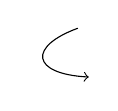
\begin{tikzpicture}[baseline=-.5ex,x=1cm,y=1cm]\draw[->] (.48,.62) .. controls (-.15,.39) and (-.12,.04) .. (.62,0);\end{tikzpicture}}}
Graphe \inserted{multi}polygonal \inserted{(ou \uline{contour} (combinatoire))}
\[
\bigl[\quad\forall s\in S,\quad\operatorname{card}R\{s\}=2\quad\bigr]
\]

\unsure{Dualité|Densité} des \deleted{graphes polygonaux} contours (combinatoires).

\deleted{\unsure{donc|donq}} les composantes \inserted{\unsure{connexes|conn.}} d'un \deleted{graphe polygonal}\inserted{contour} sont \deleted{polygonales.} des contours.

Classification des \deleted{graphes polygonaux}\inserted{contours} conn. $\ne\varnothing$

\uline{Prop} Un \deleted{graphe polyg.}\inserted{contour} connexe \inserted{$\ne\varnothing$} est connu à isom. près quand on connait $\operatorname{card}S$ ($=\operatorname{card}A$), qui est n'importe quel cardinal \deleted{fini ou infini}
\[
2\le c\le\aleph_{0}
\]
(strict sss $c\ne2$ i.e. $c\geqslant3$)
% archive sheet number: 4
\scanpage{6}
Ils correspondent aux sous-groupes \inserted{$H$} de $\mathbb{Z}$, distincts de $\mathbb{Z}$ ($c=\operatorname{card}\mathbb{Z}/H$).....

\uline{Orientation d'un contour} : \deleted{\unsure{Ch.|En.}}

\uline{Prop} Soit\deleted{\unsure{s|x}} $X=(S,A,R)$ un contour \deleted{\unsure{strict}} connexe $\ne\varnothing$.

\noindent\begin{minipage}[t]{.28\linewidth}
\figure{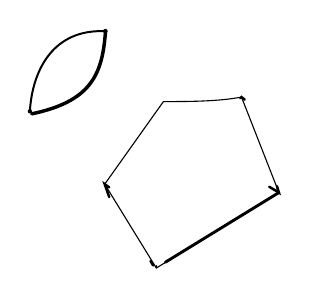
\begin{tikzpicture}[x=.0082cm,y=-.0082cm,line cap=round]
\draw[line width=.72pt] (5,126) .. controls (9,60) and (43,-2) .. (122,2);
\draw[line width=1.25pt] (122,5) .. controls (117,71) and (98,111) .. (8,130);
\fill (5,126) circle[radius=3.4]; \fill (122,2) circle[radius=3.7];
\draw (121,239) -- (212,111) .. controls (249,111) and (297,111) .. (333,104)
  -- (391,252) -- (201,369) -- cycle;
\draw[line width=1.05pt] (215,360) -- (391,252);
\draw[line width=.9pt] (128,244)--(121,239)--(128,259)
  (331,106)--(333,104)--(338,108) (376,243)--(391,252)--(388,242)
  (192,358)--(196,365);
\fill (201,366) circle[radius=1.8];
\end{tikzpicture}}
\end{minipage}\hfill
\begin{minipage}[t]{.68\linewidth}

a) \deleted{Un}\inserted{Soit $g$ un} autom. $g$ de $X$ \deleted{est dit \uline{\unsure{direct}}.}\inserted{Conditions équiv.}
\deleted{\uline{d'orientation}}

$1^{\circ})$ \deleted{\unsure{si}} $\forall s\in S$, $s$ est lié à $gs$

$2^{\circ})$ $\forall a\in A\quad ga$ est lié à $a$

\deleted{\unsure{$\{$|$f$}}

\deleted{\unsure{b)|Si}} On dit que $g$ est une \deleted{\unsure{autom.} d'}\uline{orientation} de $X$.
\end{minipage}

b) Soit $\unsure{\omega|w}(X)$\inserted{$\subset\operatorname{Aut}(X)$} l'ens des \deleted{autom. d'}orientations de $X$

Si $g\in\omega(X)$, on a $g^{-1}\in\omega(X)$.

Alors $\operatorname{card}\omega(X)=2$ \unsure{;|,} \deleted{et si $g\in\unsure{\omega|\omega(X)}$} \inserted{(si $X$ est strict i.e. si $\unsure{c|(}=\operatorname{card}S\ne2$)} , et si $g\in\omega(X)$, on a $\omega(X)=\{g,g^{-1}\}$.

c) \deleted{Soit $\operatorname{Aut}^{+}(X)\subset\operatorname{Aut}(X)$ le ss-grpe de $\operatorname{Aut}X$ formé par les $g\in\operatorname{Aut}X$ tels que $g$ opère \unsure{triv$^{\mathrm{lt}}$|triv$^{\mathrm{t}}$} sur $\omega(X)$ [i.e.}

Considérons $\operatorname{Aut}(X)\unsure{-|\to}\operatorname{Aut}(\omega(X))\simeq\mathbb{Z}/2\mathbb{Z}$.

C'est un hom surjectif, i.e. le noyau $\operatorname{Aut}^{+}(X)$ est un ss-grpe d'indice $2$.

De plus, $\operatorname{Aut}^{+}(X)$ est un groupe cyclique engendré par \unsure{tt|tout} $g\in\omega(X)$.

\uline{Corollaire} $\operatorname{Aut}(X)\simeq\mathbb{Z}/2\mathbb{Z}\cdot\mathbb{Z}/H$ \inserted{(produit $\frac{1}{2}$ direct):}, où $H$ est le ss-grpe de $\mathbb{Z}$ formé des $n\in\mathbb{Z}$ tels que $g^{n}=1$ ($g$ \unsure{étant|étans|etant} une orientation \unsure{fixé|fixée})
% archive sheet number: 5
\scanpage{7}
\uline{connexe} \uline{orienté} ``revient au $=$'' que de se donner un $n\in\mathbb{N}$, $n\geq\unsure{2|?}$, et un \inserted{tel} torseur sous $\mathbb{Z}/n\mathbb{Z}$ (savoir $S$, ou $A$ au choix -- NB $\unsure{\sigma|r}:S\longrightarrow A$ est compatible avec l'action de $G^{\unsure{0|\circ}}=\mathbb{Z}/n\mathbb{Z}$ i.e. avec l'action de $u_{\unsure{\omega|w}}$.

Se donner un \uline{contour connexe} équivaut : la donnée de

$1^{\circ})$ un \unsure{gpe|grpe} cyclique $G^{0}$ (d'ordre $n\geq2$)

$2^{\circ})$ une \deleted{\unsure{ens|un}} partie de $G^{0}$ \deleted{formée d'} de la forme $\{g,g^{-1}\}$, où $g$ est un générateur \inserted{(\unsure{donc} partie de card $2$ \unsure{sss|ss} $n\ne2$)}

$3^{\circ})$ Un torseur $S$ sous $G^{0}$

$\bullet$ Du moins si $n\geq3$ \deleted{\unsure{sinon|si on}} ; pour une description

$\bullet$ générale, il faut de plus se donner, en lieu du $2^{\circ}$, un

$2$ bis) un ens $\Omega$ à deux \unsure{élémts|éléts|éléments}, et une application $\Omega\xrightarrow{i}G$ telle que, si $\Omega=\{a,b\}$, on ait $i(a)i(b)=1$, $i(a)$ gén. de $G$

\begin{center}\rule{1cm}{.35pt}\end{center}

Contour orienté (pas \unsure{néc.|néc} connexe) $=$ ensemble sur lequel $\mathbb{Z}$ opère (i.e \unsure{avec|ou} autom \unsure{$u$|$n$})

Contour (pas néc connexe) $=$ \unsure{\ldots|un}
% archive sheet number: 6
\scanpage{8}
Orientation d'un contour.

Choix pour \unsure{tte|les|toute} arête $a\in A$ d'une ``orientation de $a$'' i.e. d'une origine $\deleted{\unsure{o|\omega}}\sigma(a)$ de $a$, de telle façon que l'on ait

% slanted
\margin{\diagram{\begin{tikzcd}[ampersand replacement=\&,column sep=small] A \arrow[r,"{\substack{\sigma\\[-.35ex]\sim}}"] \& S \end{tikzcd}}
$\forall a\in A,\ \deleted{\unsure{\exists1|\exists}}(\sigma(a),a)\in R$\\
\deleted{$\unsure{\forall s\in S|\forall a\in S},\exists1\,a\in A,$}}

\[
\begin{aligned}
&\text{Si}\quad \deleted{R\{s\}=\{a,b\},\ \text{alors }\exists}\quad s\in S,\quad \exists1\ a\in R\{s\}\ \text{tel que}\\
&s=\sigma(a).
\end{aligned}\tag*{(\unsure{O|0})}
\]

Réduction au cas connexe

\uline{Prop} Si $(S,A,R)$ est un contour connexe, il a exactement \uline{deux} orientations ($\unsure{\omega|w}$ et $-\omega$).

\figure{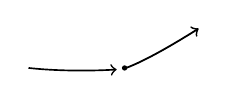
\begin{tikzpicture}[x=.02cm,y=.02cm]
\draw[->,line width=.6pt] (0,0) .. controls (18,-2) and (39,-2) .. (56,-1);
\fill (61,0) circle[radius=1.7];
\draw[->,line width=.65pt] (62,0) .. controls (75,5) and (92,15) .. (108,25);
\end{tikzpicture}}

\figure{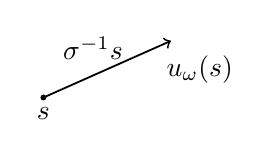
\begin{tikzpicture}[x=.03cm,y=.03cm]
\fill (0,0) circle[radius=1.25];\draw[->,line width=.65pt] (0,0)--(54,24);
\node[below] at (0,0) {$s$};
\node[above] at (21,12) {$\sigma^{-1}s$};
\node[below right] at (48,22) {$u_{\omega}(s)$};
\end{tikzpicture}}
\deleted{Prop} \uline{Prop} Soit $\omega$ orientation du contour $(S,A,R)$.

$\forall s\in S$, soit $\deleted{\unsure{\omega(s)|w(s)}\unsure{u_{\omega}|u}}\inserted{u_{\omega}}(s)$ l'\uline{extrémité} de l'unique arête \inserted{$\sigma^{-1}(s)$} qui ait \deleted{\unsure{comme}} $s$ comme origine
\[
\left[\begin{aligned}(u_{\omega}(s),\sigma^{-1}(s))&\in R,\\u_{\omega}(s)&\ne s\end{aligned}\right]
\]

\figure{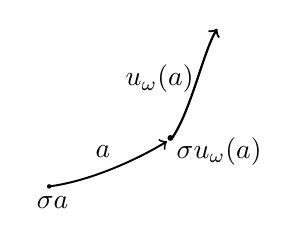
\begin{tikzpicture}[x=.022cm,y=.022cm]
\fill (0,0) circle[radius=1.3];\draw[->,line width=.7pt] (0,0) .. controls (23,3) and (50,15) .. (68,26);
\fill (70,28) circle[radius=1.7];\draw[->,line width=.8pt] (71,28) .. controls (82,44) and (89,78) .. (97,91);
\node[below] at (2,0) {$\sigma a$};\node[above] at (31,11) {$a$};
\node[right] at (68,20) {$\sigma u_{\omega}(a)$};\node[left] at (89,62) {$u_{\omega}(a)$};
\end{tikzpicture}}
$\forall a\in A$, soit $u_{\omega}(a)$ l'unique \unsure{arc|ar} de $S$ dont l'origine soit l'extrémité de $a$
\[
\left[\begin{aligned}
(\sigma u_{\omega}(a),a)&\in R,\quad \sigma u_{\omega}(a)\ne\sigma a\\
&\hspace{6em}\text{i.e.}\quad u_{\omega}(a)\ne a
\end{aligned}\right]
\]

\margin{$\big\}$}Alors $u_{\omega}:(S,\deleted{\unsure{R|B}}A)\unsure{-|\to}(S,A)$ est un autom du graphe $(S,A,R)$. On a $u_{-\omega}=u_{\omega}^{-1}$. Les autom $u_{\omega},u_{\omega}^{-1}$ sont caractérisés par les \deleted{fait que} conditions équivalentes

$1^{\circ})$ $\forall s\in S$, $s$ lié à $gs$

$2^{\circ})$ $\forall a\in A$, $a$ lié à $ga$

Si $n=\operatorname{card}S=\operatorname{card}A$, l'ordre de $u_{\omega},u_{\omega}^{-1}=u_{-\omega}$ est $n$

\unsure{flèche|et} $u_{\omega}\ne u_{-\omega}$ sss $n\ne2$ i.e. $n\geq3$ ; \unsure{donc|alors} $\omega\longmapsto u_{\omega}$ est bijection de $\unsure{\operatorname{or}|{\rm Or}}(S,A,R)$ \unsure{avec|sur} l'ens des $g\in\operatorname{Aut}(S,A,R)$ satisfaisant les conditions équiv. \unsure{$1^{\circ}$ ou $2^{\circ}\big\}$|$1^{\circ}$ ou $2^{\circ})$}, Et le \unsure{gpe|grpe} cyclique $\simeq\mathbb{Z}/n\mathbb{Z}$ engendré par $u_{\omega}$ est \deleted{\unsure{formé|form}} \inserted{le} \inserted{gpe $G^{\unsure{0|\circ}}$} des autom \inserted{orientés} de $(S,A,R,\omega)$ \inserted{\unsure{lire|les} de $S,A,R;\omega)$}. $S$ et $A$ sont des \uline{torseurs} sous $G^{0}$.

\deleted{Se donner un}

Torseur sous $\mathbb{Z}/n\mathbb{Z}$ \inserted{$(n\geq1)$} $=$ ensemble \deleted{\unsure{où}} à $n$ \unsure{élément|éléments} muni d'un ordre \unsure{$^{\times}$|$^{*}$} circulaire. Se donner un contour
% archive sheet number: 7
\scanpage{9}
1) \uline{Ens. avec permutation} $(E,u)\Longleftrightarrow\mathbb{Z}$-ens.

Classification : famille de cardinaux associés aux ss-groupes de $\mathbb{Z}$
\[
=\text{famille de cardinaux}\quad (\unsure{a|n}_{i})_{i\in\mathbb{N}}
\]

\[
E\ \text{fini}\Longleftrightarrow
\underbrace{n_{0}=0}_{\substack{\text{orbites}\\\text{finies}}}
\ \text{et}\quad
\underbrace{\text{les } n_{i}\ \text{finis}}_{\substack{\text{nb fini d'}\\\text{orbites de}\\\text{cardinal } i\in\mathbb{N}\\\text{donné}}},
\quad\underbrace{\text{nuls sauf un nb fini}}_{\text{nb fini d'orbites}}
\]

$u$ transitif ($\Longleftrightarrow u$ définit sur $E$ un ordre circulaire) $\unsure{\Leftarrow|\Leftrightarrow}$ tous les $n_{i}$ sauf un au plus sont nuls

\noindent\begin{tabular}{@{}|@{\hspace{.6em}}p{\dimexpr\linewidth-1em\relax}@{}}
\uline{Cor} Les classes d'éléments de $\unsure{\mathfrak{S}|\mathscr{S}}_{n}$ mod conjugaison correspondent $1$-$1$ aux ``partitions'' de $n$, i.e. aux familles d'entiers $(c_{i})_{1\leq i\leq n}$ tels que
\[
\sum i c_{i}=n
\]
\end{tabular}

\diagram{\resizebox{\linewidth}{!}{\begingroup\setlength{\arraycolsep}{2.5pt}\(\begin{array}{ll l|ll l}
\mathfrak{S}_{2}:&2\ \text{classes}&1,\sigma_{12}&\unsure{\mathfrak{A}|\mathscr{A}}_{2}:&1\ \text{classe}&1\\
\mathfrak{S}_{3}:&3\ \text{classes}&1,\sigma_{12},\sigma_{123}&\mathfrak{A}_{3}:&3\ {-}&1,\sigma_{123},\sigma_{321}\\
\mathfrak{S}_{4}:&5\ \text{classes}&1,\sigma_{12},\sigma_{12}\sigma_{34},\sigma_{123},\sigma_{1234}
&\mathfrak{A}_{4}:&\multicolumn{2}{l}{\tikz[baseline=(entry.base)]{
  \node[inner sep=1.5pt] (entry) {$\deleted{\unsure{1|i},\sigma_{\unsure{12|13}}\sigma_{\unsure{34|24}},\sigma_{\unsure{1234|4234}}}$};
  \draw[rounded corners=2.5pt] ([xshift=-2em,yshift=1.5pt]entry.north east)
    -- ([xshift=-2em]entry.north east) -- (entry.north west) -- (entry.south west)
    -- ([xshift=-1.65em]entry.south east) -- ([xshift=-1.65em,yshift=-1.5pt]entry.south east);
}}\\
\mathfrak{S}_{5}:&?&&&&
\end{array}\)\endgroup}}

2) \uline{Rectification} Les contours orientés correspondent aux ens. à permutation $(E,u)$ tels que $u$ n'\uline{ait pas de pt fixe} (car on ne veut pas de polygone à $1$ coté, ds les graphes !)

3) Produit $\frac{1}{2}$ direct de gpes

donner
\diagram{\begin{tikzcd}[ampersand replacement=\&,column sep=small]
1 \arrow[r,dash] \& \unsure{\mathbb{Z}|Z}\arrow[r,dash,"i"] \& G\arrow[r,dash,"p"] \& \Gamma\arrow[l,bend left=24,"q"']\arrow[r,dash] \& 1\unsure{q} \&[-1ex] \unsure{p|q}qp=\operatorname{id}_{\Gamma}\quad\unsure{q|p}
\end{tikzcd}}
(suite exacte, avec $q$ un hom. de groupes)

revient à donner
\diagram{\begin{tikzcd}[ampersand replacement=\&,column sep=small,row sep=0pt]
1\arrow[r,dash] \& Z\arrow[r,dash] \& G\arrow[r] \& \Gamma\arrow[r,dash] \& 1 \& p\mid\Gamma'\simeq\deleted{\unsure{\mathrm{iso}|\mathrm{is}}}\Gamma\ \text{\unsure{iso|is}}\\
\& \& \rotatebox{90}{$\subset$} \\
\& \& \Gamma'
\end{tikzcd}}

ou à donner \unsure{gpes|grs} $Z,\Gamma$ avec op. de $\Gamma$ sur $Z$
\[
\Gamma\longrightarrow\operatorname{Aut}_{\unsure{\mathrm{gr}|\mathrm{gr.}}}(Z)
\]

loi de composition sur $G=\mathbb{Z}\times\Gamma$

% slanted
\margin{\unsure{Parler|parler} ici d'un \unsure{gr|gpe} \unsure{inverseur|inverseurs} d'extensions \unsure{car|où} cela permet d'introduire $\operatorname{Aff}(Z)\simeq Z\cdot\operatorname{Aut}Z$ \deleted{\unsure{Aut|Aut(Z)}}.}

\[
\begin{aligned}
&\deleted{(\gamma,z)(\gamma',z')=(\gamma\gamma',\operatorname{int}(\gamma')^{-1}(z)\cdot z')}\\
&(z,\gamma)(\unsure{z'|{\mathcal Z}'},\gamma')=(z\operatorname{int}(\gamma)(z'),\gamma\gamma')
\end{aligned}
\]

\margin{Ss-groupes $G'$ de $G$ avec $G'\supset Z$ $\Longleftrightarrow$ ss-gpe $\Gamma'$ de \deleted{\unsure{$\Gamma$|$R$}} et on a $G'\simeq\mathbb{Z}\cdot\Gamma'$ ($\frac{1}{2}$ direct)}
% archive sheet number: 8
